%%%%%%%%%%%%%%%%%%%%%%%%%%%%%%%%%%%%%%%%%%%%%%%%%%%%%%%%%%%%%%%%%%%%%%
% This layout was adapted from one found at latextemplates.com which
% was adapted from another.
%
% License: CC BY-NC-SA 3.0
% (http://creativecommons.org/licenses/by-nc-sa/3.0/)
%
% Original header:
%
% This is a LaTeX version of the sample laboratory report from
% Virginia Tech's copyrighted 08-09 CHEM 1045/1046 lab manual.
% Reproduction of this one appendix section for academic purposes
% should fall under fair use.
%
%%%%%%%%%%%%%%%%%%%%%%%%%%%%%%%%%%%%%%%%%%%%%%%%%%%%%%%%%%%%%%%%%%%%%%

\documentclass{article}

\usepackage{graphicx}
%\usepackage[acronym]{glossaries} % Lets us use acronyms
\usepackage{siunitx} % SI units in math mode

\author{}
\title{ELEC-313 \\ Lab 2: Diode Characterization \\ }
\date{\today}

%\loadglsentries{acronyms} % Actually loads 'acronyms.tex'
%\makeglossaries

\begin{document}

\maketitle

\begin{center}
  \begin{tabular}{lr}
    Date Performed: & September 18, 2013 \\
    Partners: & Charles Pittman \\
    & Stephen Wilson \\
  \end{tabular}
\end{center}

\pagebreak

% Removes indentation from paragraphs: \setlength\parindent{0pt}

% Number the enumerate environment (unordered lists) by letter:
\renewcommand{\labelenumi}{\alph{enumi}.}

\section{Objective}
\label{sec:objective}


\section{Schematics}
\label{sec:schematics}

% The asterisk after section inhibits the numbering of the section.
\subsection*{Circuit Tested}
\label{sec:ckt_tested}

%\begin{figure}[hbtp]
%  \centering
%    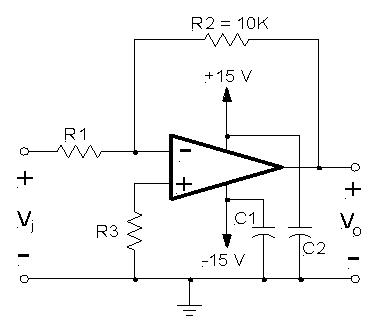
\includegraphics[]{img/ckt_tested}
%  \caption{\label{fig:circuit} Circuit being tested.  $C_1 = C_2 = \SI{1}{\micro\farad}$}
%\end{figure}

\subsection*{Test Configuration}
\label{sec:test_config}

%\begin{figure}[hbtp]
%  \centering
%  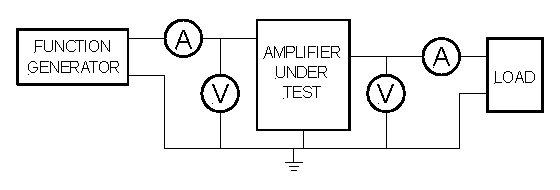
\includegraphics[]{img/test_config}
%  \caption{\label{fig:test_config} Test Configuration}
%\end{figure}

\section{Procedure}
\label{sec:procedure}

%First, resistors $R_1$, $R_2$, and $R_3$ were measured with a
%multimeter and recorded in Table~\ref{tab:table_01}.  Then the circuit
%in Figure~\ref{fig:circuit} was constructed on a breadboard.  Next,
%the configuration depicted in Figure~\ref{fig:test_config} was assembled.
%
%Two Fluke multimeters served as the ammeters, and two input channels
%of an oscilloscope served as voltmeters.  The function generator was
%set to produce a sine wave with amplitude of
%\SI{200}{\milli\volt_{rms}} @ \SI{1}{\kilo\hertz}, serving as the
%voltage source, and a decade box set to \SI{200}{\ohm} serving as the
%load.
%
%With the load disconnected, the input voltage ($V_i$), input current
%($I_i$), output voltage ($V_o$), and output current ($I_i$) were
%measured and recorded in Table~\ref{tab:table_02}.  This step was then
%repeated with the load connected.  Using these values with the
%equations derived from the four amplifier models, measured values were
%determined where direct measurement was difficult.

\section{Results}
\label{sec:results}

\subsection{Part A}
\label{sec:result_a}

% This LaTeX table template is generated by emacs 24.3.1
\begin{tabular}{|l|l|l|}
  \hline
  -5.00 & -5.000 & 0.01 \\
  \hline
  -4.50 & -4.500 & 0.01 \\
  \hline
  -4.00 & -4.000 & 0.01 \\
  \hline
  -3.50 & -3.500 & 0.01 \\
  \hline
  -3.00 & -3.000 & 0.01 \\
  \hline
  -2.50 & -2.500 & 0.01 \\
  \hline
  -2.00 & -2.000 & 0.01 \\
  \hline
  -1.50 & -1.500 & 0.01 \\
  \hline
  -1.00 & -1.000 & 0.01 \\
  \hline
  -0.50 & -0.500 & 0.01 \\
  \hline
  0.00 & 0.277 & 0.01 \\
  \hline
  0.25 & 0.254 & 0.01 \\
  \hline
  0.50 & 0.461 & 0.10 \\
  \hline
  0.75 & 0.536 & 0.46 \\
  \hline
  1.00 & 0.570 & 0.92 \\
  \hline
  1.25 & 0.591 & 1.40 \\
  \hline
  1.50 & 0.606 & 1.89 \\
  \hline
  1.75 & 0.618 & 2.39 \\
  \hline
  2.00 & 0.627 & 2.90 \\
  \hline
  2.25 & 0.635 & 3.41 \\
  \hline
  2.50 & 0.642 & 3.92 \\
  \hline
  2.75 & 0.648 & 4.44 \\
  \hline
  3.00 & 0.653 & 4.95 \\
  \hline
  3.25 & 0.658 & 5.47 \\
  \hline
  3.50 & 0.662 & 5.99 \\
  \hline
  3.75 & 0.666 & 6.51 \\
  \hline
  4.00 & 0.670 & 7.03 \\
  \hline
  4.25 & 0.673 & 7.55 \\
  \hline
  4.50 & 0.676 & 8.08 \\
  \hline
  4.75 & 0.679 & 8.60 \\
  \hline
  5.00 & 0.682 & 9.13 \\
  \hline
  5.50 & 0.687 & 10.18 \\
  \hline
  6.00 & 0.692 & 11.23 \\
  \hline
  6.50 & 0.696 & 12.30 \\
  \hline
  7.00 & 0.699 & 13.36 \\
  \hline
  7.50 & 0.703 & 14.42 \\
  \hline
  8.00 & 0.706 & 15.49 \\
  \hline
  8.50 & 0.709 & 16.56 \\
  \hline
  9.00 & 0.712 & 17.66 \\
  \hline
  9.50 & 0.714 & 18.75 \\
  \hline
  10.00 & 0.717 & 19.84 \\
  \hline
\end{tabular}

\section{Conclusion}
\label{sec:conclusion}

As shown in Table~\ref{tab:table_03}, the amplifier models do closely
represent the amplifier used in the experiment.  The greatest
difference occurred in the current gain ($A_i$), largely due to $R_o$
being nearly zero.  This also causes $G_m$ to be very large.

\section{Appendix}
\label{sec:appendix}

\subsection*{Equations}

% LaTeX sees blank lines as a start of another paragraph.  To avoid
% unnecessary vertical spaces between equations, and still visually
% separate in source, put a comment between them.
\begin{equation}
  \label{eqn:percent_error}
  \%_{error} = \frac{|measured - nominal|}{nominal} \times 100\%
\end{equation}
%
\begin{equation}
  \label{eqn:R_o}
  R_o = \frac{V_{noload} - V_{load}}{I_{load}}
\end{equation}
%
\begin{equation}
  \label{eqn:R_i}
  R_i = \frac{V_i}{I_i}
\end{equation}
%
\begin{equation}
  \label{eqn:A_v}
  A_v = \frac{V_o}{V_i}
\end{equation}
%
\begin{equation}
  \label{eqn:A_i}
  A_i = A_v \left(\frac{R_i}{R_o}\right)
\end{equation}
%
\begin{equation}
  \label{eqn:G_m}
  G_m = \frac{A_v}{R_o}
\end{equation}
%
\begin{equation}
  \label{eqn:R_m}
  R_m = A_v R_i
\end{equation}

\end{document}
